\chapter{Proof of concept}
\label{ch:poc}


In dit hoofdstuk wordt de proof of concept besproken, op basis van de resultaten van bovenstaande literatuurstudie. Hier wordt stap voor stap de testopstelling en installatie van de classroom management software uitgeschreven. De software die werd gekozen in de literatuurstudie is de open-source software Veyon. Deze software tool komt met zijn groot aantal voordelen er als beste uit in deze casus. 

\section{Doelstelling en vereisten}
De proof of concept omvat de installatie van zowel de klasopstelling als het programma zelf. Tevens is het mogelijk om deze testopstelling snel en efficiënt na te bootsen. Daarnaast stellen de administrators van Veyon de minimale systeemeisen op. Ook checkt deze proof of concept de minimale systeemeisen om overtollige uitgaves uit te sparen. Tot slot wordt de software uitgebreid getest in de vooropgestelde testopstelling en worden er zo veel mogelijk functionaliteiten uitgevoerd en nagekeken.  

\section{Functionaliteiten}
Vooraleer er verder wordt gegaan in het uitwerken van de proof of concept, is het belangrijk om de achtergrond functionaliteiten te beschrijven van Veyon. Hieronder worden enkele belangrijke IT gerichte functionaliteiten beschreven. Deze functionaliteiten zijn belangrijk voor een veilige connectie tussen de computers van de leerkracht en de leerlingen. Door gebruik te maken van de officiële documentatie van Veyon \textcite{VeyonFunctionaliteiten} is onderstaande beschrijving opgebouwd.

\subsubsection{LDAP/AD integration}
Eén van de eerste opvallende functionaliteiten is het gebruik van LDAP (Lightweight directory access protocol) en AD (Active Directory) integration. Deze twee technologieën worden vaak gebruik voor directory services en identiteitsbeheer van groepen of gebruikers, maar verschillen onderling wel in functies, toepassingen en kenmerken. \newline
 
 In de documentatie van Microsoft \textcite{janicericketts-2023} wordt beschreven dat LDAP (Lightweight directory access protocol) een toepassingsprotocol is voor het werken met directoryservices. Meestal wordt hier Active Directory voor gebruikt, dienend voor het bewaren van gebruikers met hun accountgegevens zoals een e-mail adres of wachtwoorden. Zodoende kan deze service deze gegevens delen met andere computers over het netwerk.
 
 Door gebruik te maken van de integratie van LDAP (Lightweight directory access protocol) en Ad (Active Directory) in het programma Veyon kan de bestaande directory-informatie direct gebruikt worden in het netwerk. Zodoende verminderen administratieve taken sterk in tijd en waarborgt het programma de consistentie van gegevens.  
 
 \subsubsection{Authentication}
 De tweede opvallende functionaliteit van Veyon is de methode van Authenticatie. Veyon biedt twee verschillende soorten authenticatie methodes, namelijk key authentication en login authentication. Hieronder worden beide methodes uitgebreid vergeleken om zo de makkelijkste manier toe te passen in de proof of concept. \newline
 
 De eerste authenticatiemethode van Veyon die besproken wordt is Key Authentication. Deze methode volgt de asymmetrische cryptografie methode bij het aanmaken en gebruiken van sleutels, waardoor er altijd een publieke en unieke sleutel aanwezig is. Hierdoor krijgen alleen geautoriseerde gebruikers met een geldige sleutel toegang tot Veyon Master waar het verder beheer mogelijk is. Zodoende is een extra beveiliging actief waardoor het programma moeilijker aanpasbaar is. 
 
 Voor elke Master pc die wordt gegenereerd moet een sleutel worden aangemaakt. Tijdens het aanmaken kan gekozen worden voor een bijpassende naam die herkenbaar is in grote lijsten van verschillende sleutels. Wanneer deze sleutel aangemaakt is, is er een publieke en unieke sleutel aanwezig. Door deze publieke sleutel door te sturen naar de leerlingen is het mogelijk om connectie te maken met de virtuele klassen. Hierdoor kan de Master pc met de leerlingen connecteren en is het mogelijk om van start te gaan met de verdere installatie.\newline
 
 
 \textbf{Voordelen van Key authentication}
 \begin{itemize}
     \item Geen aanmelding meer nodig: wanneer deze methode gehanteerd wordt is het niet meer nodig om aan te melden met de gebruikersnaam en paswoord voor toegang te krijgen tot Veyon Master. Er wordt automatisch connectie gemaakt waardoor het inloggen sneller in werking treedt. 
     \item Centraal beheer: deze methode zorgt voor een centrale beheermethode waarbij elke sleutel kan beheerd worden. Hierbij kunnen er extra sleutels aangemaakt, doorgestuurd of geïmporteerd worden om zo de connectie mogelijk te maken.
 \end{itemize}
  \textbf{Nadelen van Key authentication}
 \begin{itemize}
     \item Langere installatie: door gebruik te maken van deze methode is het mogelijk dat de installatie langer verloopt. Ook moet er extra IT kennis aanwezig zijn voor deze methode tot een goed einde te configureren.
     \item Geen extra controle: wanneer de sleutel is geconfigureerd is er geen extra controle mogelijk. Waarbij elke persoon op elke computer kan inloggen en deelnemen aan de virtuele klas. Dit kan zorgen voor een zwakke beveiliging wanneer de computers naar huis worden meegenomen.
     \item Veranderingen nodig bij wijzigen privésleutel: wanneer de privésleutel gewijzigd wordt om bepaalde redenen, moeten alle andere publieke sleutels worden aangepast voor wederzijdse connectie. Dit kan zorgen voor extra moeilijkheden voor de administrator of IT-personeel op de scholen.
 \end{itemize}
 De tweede authenticatiemethode van Veyon die besproken wordt is Login authentication.
 Deze methode versleutelt de Veyon master, de gebruikersnaam en het wachtwoord van de leerkracht die probeert in te loggen. Vervolgens worden de gegevens doorgestuurd naar de Veyon service op de remote computer. Nadien wordt er intern aangemeld op de lokale computer waar Veyon Master actief is door gebruik te maken van de gedecodeerde sleutel. Wanneer de aanmeldingsprocedure succesvol verlopen is, krijgt diegene toegang tot de Veyon Master. Indien de verbinding mislukt, wordt deze aanmelding verworpen en eveneens de verbinding gesloten.
 
 Deze methode is alleen zinvol wanneer identieke gebruikersaccounts op alle computers aanwezig zijn. Dit komende door het gebruik van centrale gebruikersdirectory die gehanteerd worden in de LDAP/AD integration. 
 
 Om een betere beslissing te maken welke authenticatie methodes in deze casus het beste van toepassing zijn, worden er voor beide voor- en nadelen opgesomd. Daarna kan deze methode in deze proof of concept uitgewerkt en geïmplementeerd worden.\newline
 
 \textbf{Voordelen Login authentication}
 \begin{itemize}
     \item Eenvoudige installatie: deze methode omvat geen complexe sleutelbeheer, waardoor deze installatie sneller verloopt.
     \item Extra controle: wanneer een gebruiker wil inloggen op het systeem moet deze zijn gebruikersnaam en wachtwoord opgeven. Hierdoor wordt er altijd gecontroleerd of deze persoon de toegang tot de Veyon Master mag verschaffen.
 \end{itemize}
  \textbf{Nadelen Login authentication}
 \begin{itemize}
     \item Aanmelding vereist: Wanneer Veyon Master wordt opgestart moet de leerkracht elke keer de gebruikersnaam en paswoord ingeven. Dit verlengt het proces tijdens de lessen, wat niet de bedoeling is.
 \end{itemize}
 
 Bovenstaande voor- en nadelen tonen aan dat beide methodes goede opties zijn om geautoriseerde toegang te garanderen. Toch wordt er in deze casus gekozen voor het gebruik van Key authentication, omdat er meer aandacht aan gebruiksgemak en efficiëntie wordt besteed. Hoewel de installatie van deze methode meer aandacht en configuratie vraagt, kan deze methode tijdens de lessen de stressfactor van de leerkrachten reduceren en is er nog altijd aandacht voor een robuuste beveiliging. Ook is het niet van toepassing dat leerlingen zomaar de Master pc van de leerkracht kunnen bereiken. Om deze reden verdwijnt het grote voordeel bij Login authentication.  
 
 \subsubsection{Access control}
 
 Vervolgens komt de functionaliteit Access control aan bod, die garant staat voor de gecontroleerde toegang van specifieke gebruikers. Deze functie is zeer nuttig in omgevingen waar meerdere klassen of groepen tegelijkertijd worden beheerd. Door gebruik te maken van deze functie kunnen administrators instellen welke computers er tot welke groep behoren en hoe deze groepen toegang krijgen tot verscheidene functionaliteiten.
 
 In deze casus is het gebruik van Access control niet van toepassing. Deze functie zou het omslachtig maken voor de installateur omdat niet elke leerling een laptop op school te beschikking heeft. De scholengroep voorziet kasten met laptops, maar deze laptops zijn beperkt waardoor leerkrachten deze moeten reserveren. Dit wil zeggen dat niet elke leerling een afzonderlijke computer tot zijn beschikking heeft. Wat resulteert in het niet verder uitwerken van de Access control functie in de proof of concept.
 
\section{Ontwikkeling}
\subsection{Creëren klasopstelling}
\label{creërenklasopstelling}
Door de uitwerking van de literatuurstudie is er geweten dat Veyon op zowel Linux als Windows besturingssystemen draait. Omdat Linux op weinig tot geen school wordt gehanteerd, beperkt deze proof of concept zich alleen tot de installatie op Windows machines. Zodoende wordt de klasopstelling gemaakt met 4 Windows 10 machines. \newline

Voor de klasopstelling te creëren is een ISO file essentieel. Deze ISO file is een digitaal bestand dat een systeem omgeving repliceert. Zo kan de gehele Windows 10 omgeving worden geïnstalleerd en geconfigureerd. Via een schoolaccount kan deze gratis worden geïnstalleerd op de website van Academic Software\footnote{\url{https://portal.academicsoftware.com/dashboard}}. Het is belangrijk de Windows 10 Pro Education 64bit\footnote{\url{https://portal.academicsoftware.com/software/windows-10-education~43084e96-9c0a-479b-b877-8cdf155399f7}} te installeren. Het is overbodig de ISO file voor elke machine te downloaden omdat deze na de volledige doorloop wordt losgekoppeld van de machine zelf. \newline

Volgens de handleiding van \textcite{veyonrequirements} zijn er minimale systeemeisen waaraan de apparaten moeten voldoen, voor een succesvolle installatie. Hieronder worden deze kort beschreven:
\begin{itemize}
    \item Minstens 2GB RAM geheugen (Hoe meer leerlingen er zijn hoe meer RAM geheugen er moet vrijgemaakt worden. Betrekkend tot het bekijken van de schermen van leerlingen)
    \item Multi-core CPU (is een CPU die over meer dan één kern beschikt, in dit geval is de minimum vereiste 2 tot 4 CPU cores)
    \item Besturingssysteem: \begin{itemize}
        \item Windows 10 of 11 (32/64bit)
        \item Verschillende Linux distributies zoals Debian, Ubuntu, openSUSE, Fedora en CentOS   
    \end{itemize}
\end{itemize}

Er wordt uitsluitend gesproken over de minimale systeemeisen voor de Master pc, terwijl er geen informatie wordt gegeven over de minimale systeemeisen voor de Client pc. Om ervoor te zorgen dat alles correct functioneert, draaien de virtuele machines in een Virtualbox 7.0 omgeving waar volgende systeemconfiguratie gelden, zie figuur \ref{fig:Vereisten virtuele machines POC}. 

\begin{figure}[h]
     \centering
     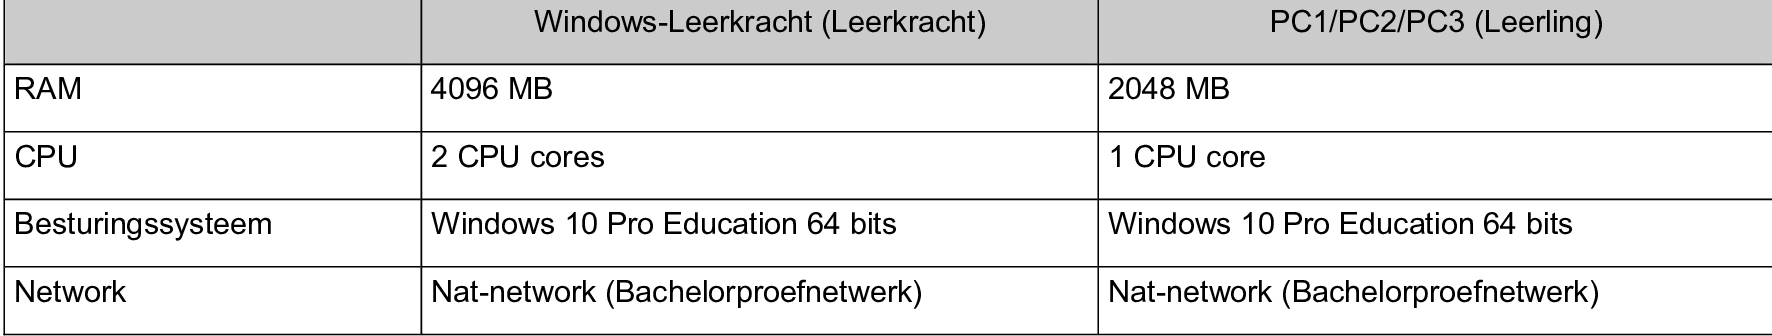
\includegraphics[width=1\textwidth]{graphics/vereisten.png}
     \caption{Gebruikte vereisten virtuele machines POC}
     \label{fig:Vereisten virtuele machines POC} 
\end{figure}

Bovenstaande figuur \ref{fig:Vereisten virtuele machines POC}, toont aan wat er in deze proof of concept is gehanteerd. Wanneer er wordt gekeken in het dagelijkse leven is het niet relevant om hiervan uit te gaan. Alle hedendaags computers beschikken doorgaans over meer RAM (Random-acces memory) dan hier in de casus wordt vertoont. Echter is het niet gebruikelijk dat alle beschikbare RAM van een computer exclusief wordt toegewezen aan één programma, zoals Veyon. Kenmerkend aan RAM is dat het wordt gedeeld tussen verscheidene programma's en processen, waaronder noodzakelijke systeemtaken en andere gebruikersapplicaties zoals Google.

Naast het RAM-geheugen, dat verantwoordelijk is voor het tijdelijk opslaan en ophalen van gegevens tijdens de uitvoering van een programma, speelt de CPU (central proccesing unit) ook een belangrijke rol in het verwerken van instructies gedurende de uitvoering van een programma. Een van de belangrijkste aspecten van de CPU is het aantal 'cores', ook wel kernen genoemd, die beschikbaar zijn. Dit betrekt zich tot de limit van uitvoeringen die de CPU tegelijkertijd aankan. Wat wil zeggen, hoe meer kernen of 'cores' er beschikbaar zijn hoe sneller de taken worden uitgevoerd. In deze casus is het niet van toepassing extra kernen te voorzien naast het minimum. Dit omdat de proof of concept zich alleen maar richt tot het testen en configureren van deze tool. Waardoor het minimum aan vereisten voldoende is.\newline

Om de Windows 10 omgeving volledig op te starten en te installeren, is het van groot belang de vooropgestelde stappen van Windows zelf te doorlopen. Wanneer alle stappen gevolgd worden kan het verdere vervolg van de proof of concept doorlopen worden.

\subsubsection{Standaard configuratie van virtuele machines}
Voor de installatie van het programma Veyon repliceerbaar te maken, is het van toepassing een shared folder op te stellen. Hierdoor is het van groot belang deze toe te passen zodat bestanden van de ene virtuele machine naar de andere kunnen worden geschreven zonder veel moeite. Daarvoor is het installeren van VirtualBox Guest Additions nodig. Zodoende kan de shared folder worden configureerd. Wanneer deze proof of concept in een echte klasomgeving wordt nagebootst is het gebruik van een simpele USB-stick (Universal serial bus) voldoende. Dit hardware apparaat zorgt voor de simpele overdracht van informatie van computer naar computer.

\subsection{Installatie Veyon}
Eens de volledige installatie van de Windows machines van hoofdstuk \ref{creërenklasopstelling} is voltooid, volgt de installatie van Veyon. Deze installatie bestaat uit het installeren van de Master pc, wat betrekking heeft tot de computer van de leerkracht. Alsook de installatie van de Client pc's wat betrekking heeft tot de computers van de leerlingen. Dit hoofdstuk wordt onderverdeeld in twee delen omdat de configuratie van de Client pc's divers is. 
 

\subsubsection{Installatie Master pc}
Om de installatie van Veyon te beginnen, wordt er gestart met de installatie van de Master pc. Dit is namelijk essentieel voor toezicht te behouden op de leerlingen en beheertaken uit te voeren vanaf het apart programma Veyon Configurator. Eveneens wordt de installatie onderverdeeld in twee hoofdstukken, namelijk de standaard installatie en daarna de installatie en configuratie van de add-ons.\newline 

Allereerst wordt Veyon geïnstalleerd via de officiële website van Veyon\footnote{\url{https://veyon.io/en/}} zelf. Op dit moment van schrijven, 7 mei 2024, is Veyon versie 4.8.3.0 actief. Het is belangrijk om de versie correct te hanteren omdat de add-ons dezelfde versie volgen. Anders kunnen moeilijkheden plaatsvinden in het vervolg van de proof of concept. Omdat de configuratie van Veyon master en Veyon client hetzelfde installatiebestand gebruiken, wordt het bestand op de shared folder gezet. Zodoende is het niet nodig om voor elke computer een nieuw bestand te installeren van de website.\newline 

Tijdens de configuratie van master pc is het belangrijk om de installatielijst te doorlopen en te lezen. Het is van uiterst belang het component Veyon Master aan te duiden. Nadien kan dit niet aangepast worden wanneer de installatielijst is doorlopen. Deze stap van de installatie wordt verduidelijkt in figuur \ref{fig:Schermafbeelding Veyon Master}.

\begin{figure}[h]
    \centering
    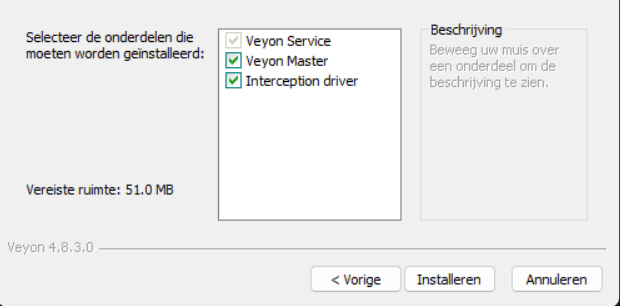
\includegraphics[width=0.75\textwidth]{graphics/SchermafbeeldingVeyonMaster.png}
    \caption{Schermafbeelding Veyon Master}
    \label{fig:Schermafbeelding Veyon Master} 
\end{figure}

Na de installatie zijn er twee verscheidene programma's geïnstalleerd, namelijk Veyon Master en Veyon Configurator. Het programma Veyon Master is bedoeld voor dagdagelijks gebruik van het programma. Hierin gaan leerkrachten het overzicht bewaren over de klas. Het andere programma is bedoeld voor de administrator, wat dit betreft worden de nodige configuratiemogelijkheden geconfigureerd. \newline

\textbf{Authentication}\newline
Eén van de belangrijkste keuzes tijdens de configuratie van Veyon is authentication. De twee mogelijkheden die kunnen gekozen worden zijn Key Authentication en Login Authentication. Door beide mogelijkheden te testen in de proof of concept, is diegene met de minst complexe installatie de uitvoerbare keuze. In deze proof of concept wordt er gewerkt met de Key Authentication methode. \newline

Door deze mogelijkheid te kiezen in de proof of concept, is de configuratie eenvoudig te implementeren en kan er tegelijkertijd effectieve toegang beheerd worden tot de Veyon Master. Met deze aanpak kunnen administrators specifieke sleutels toewijzen aan verscheidene groepen of gebruikers, waardoor toegangscontrole gegarandeerd wordt. \newline

 Na het aanmaken van de authenticatie sleutel van de leerkracht (Mastercomputer) is het belangrijk de publieke sleutel op de shared folder te zetten. Hierdoor kan deze direct worden meegegeven aan de Client pc's, waardoor de installatie nog sneller verloopt. \newline
 
\subsubsection{Installatie Client pc's}

Nadat de installatie en configuratie van de Master pc is voltooid volgt de installatie van Client computers, waar de shared folder ook wordt gehanteerd. Hierdoor wordt de tijd van installeren beperkt, wat nodig is wanneer gesproken wordt van meerdere computers. Zodoende kan de administrator snel en efficiënt te werk gaan. In deze proof of concept worden er drie leerling computers gebruikt en geïnstalleerd. Dit proces volgt bij elke computer van dezelfde virtuele klas volgende installatiemethoden.\newline

Allereerst wordt het uitvoerbaar bestand op de shared folder geopend. Dit installatiebestand geeft dezelfde omgeving weer als bij de Mastercomputer. Het enige verschil met de Veyon installatie van de Mastercomputer, zit bij aankruising van de componenten in de installatielijst. Hierbij moet de selectie van het component Veyon Master ongedaan worden gemaakt, zoals figuur \ref{fig:Schermafbeelding Veyon Client} weergeeft.

\begin{figure}[h]
    \centering
    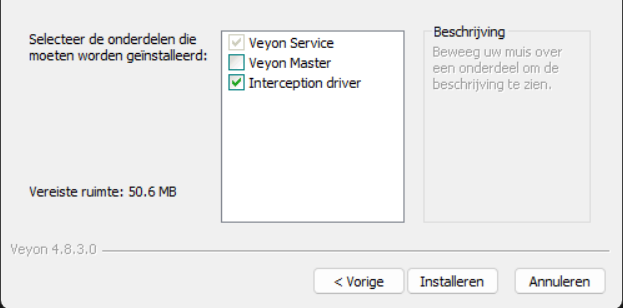
\includegraphics[width=0.75\textwidth]{graphics/SchermafbeeldingVeyonClient.png}
    \caption{Schermafbeelding Veyon Client}
    \label{fig:Schermafbeelding Veyon Client} 
\end{figure}
De installatie wordt zoals de Master pc afgerond, om daarna de authenticatie te configureren.\newline

\textbf{Authentication}\newline
De volgende stap bij het configureren van de Client pc, is het importeren van de publieke sleutel. In deze proof of concept bevindt de sleutel zich in de shared folder. Eveneens is het belangrijk bij deze sleutel dezelfde naamgeving te hanteren als op de Master pc, dit om verwarring te voorkomen. \newline

\subsubsection{Locatie en computers}
Onder de sectie 'Locatie & computers' worden de virtuele klassen aangemaakt. Hierin worden de computers geselecteerd die deelnemen aan de klas. Leerkrachten kunnen beheerder zijn van meerdere klassen tegelijkertijd, wat extra observatiemogelijkheden biedt. De computers kunnen alleen aan de klas worden gekoppeld wanneer de naamgeving van de klas overeenkomt op zowel Master als Client computer. Doordat de koppeling op meerdere manieren kan gebeuren worden er in deze proof of concept twee klassen aangemaakt namelijk 'A001' en 'B001'. Hierdoor kan er op beide koppelingsmethoden worden getest welke de makkelijkste is. \newline

Wanneer de virtuele klassen zijn aangemaakt op de Client computer kan de configuratie op de Master pc verder worden gezet. In beide klassen worden de computers toegevoegd, zo weet het programma welke computer wie is om zo het overzicht te bewaren. Tijdens de proof of concept worden bij klas 'B001' de computer gekoppeld met hun unieke naam. Waarbij klas 'A001' de computers gekoppeld worden met hun unieke naam en IP-adres. Omdat alle scholen met een DHCP (Dynamic Host Configuration Protocol) server werken is het onmogelijk unieke IP-adressen mee te geven. Deze adress worden automatisch gegenereerd door de server en aan de beschikbare apparaten gegeven. Waardoor klaslokaal 'B001' de voorkeur krijgt. Wanneer deze stap correct is uitgevoerd zijn alle toegevoegde apparaten zichtbaar op de Mastercomputer, zie figuur \ref{fig:Schermafbeelding overzicht Veyon Master}.  

\begin{figure}[h]
    \centering
    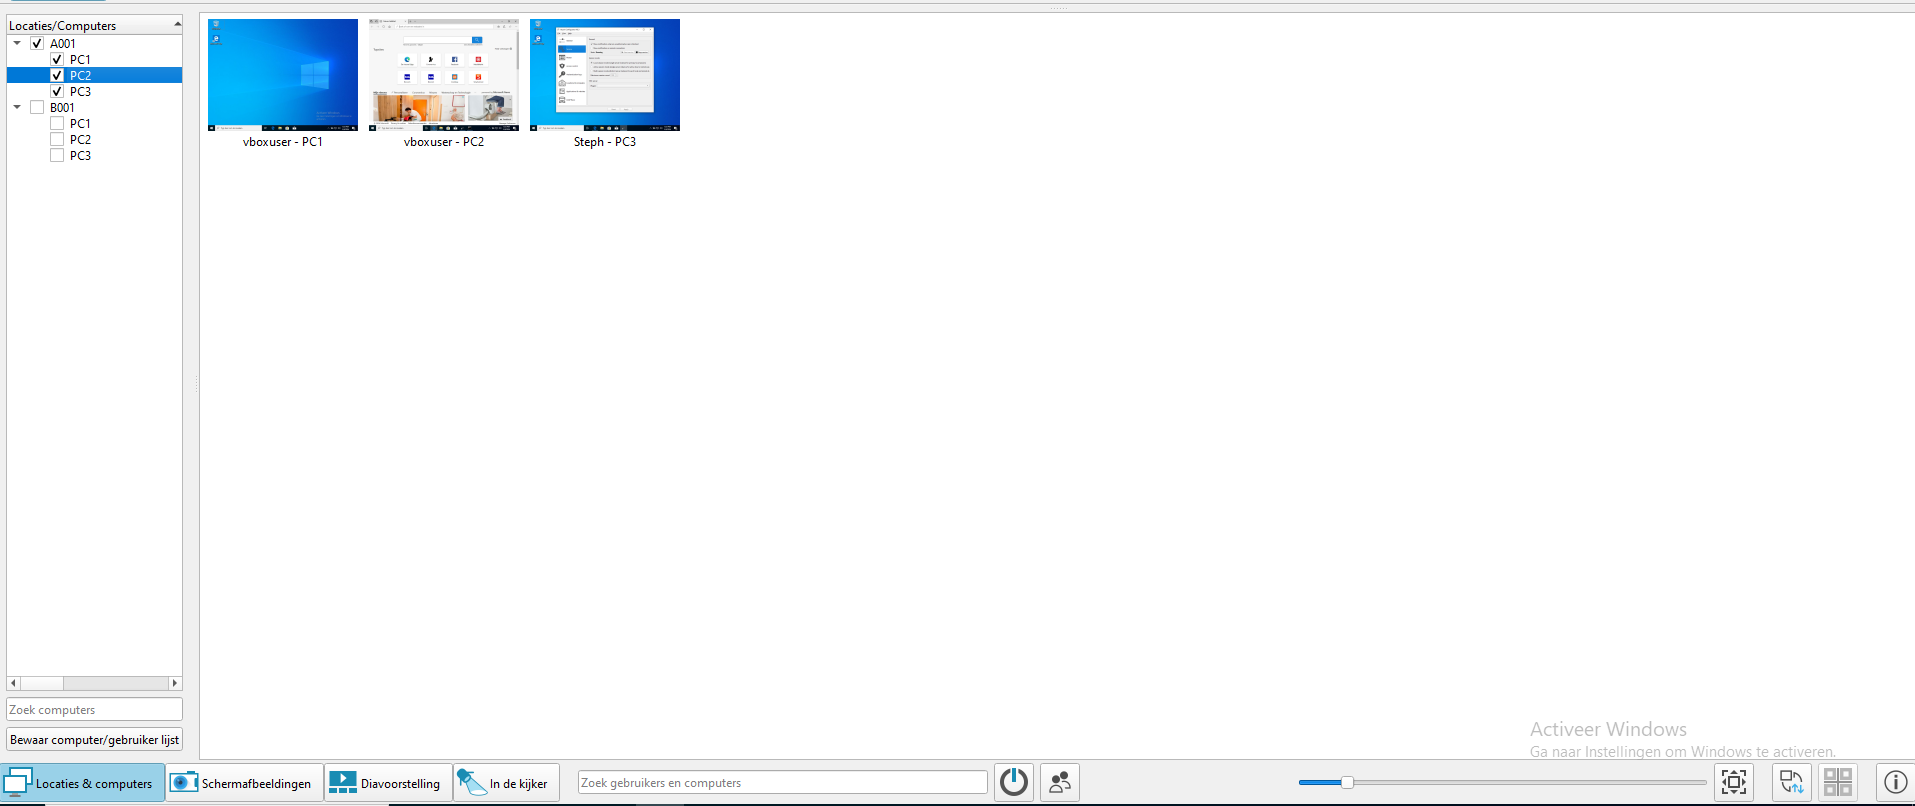
\includegraphics[width=1\textwidth]{graphics/SchermafbeeldingVeyonMasterOverzicht.png}
    \caption{Schermafbeelding overzicht Veyon Master}
    \label{fig:Schermafbeelding overzicht Veyon Master} 
\end{figure}

\subsection{Uitbreidingspakketten}
Desondanks de standaard versie van Veyon al vele functionaliteiten bezit, zijn er nog verscheidene mogelijkheden aan uitbreidingen, beter bekend als Add-ons. Dit zijn een aantal extra pakketten die te installeren zijn tegen een kleine som van betaling voor de gehele Veyon omgeving. Eén van deze pakketten betrekt zich volledig tot de uitwerking van deze casus, namelijk het filteren van websites. Onderstaande tekst werd beschreven door \textcite{junghans-2023} op de pagina van de Veyon add-ons \newline

Het voordeel van de Add-ons zit in de mogelijkheid tot het apart installeren, hierdoor is het mogelijk om bijvoorbeeld alleen het pakket van Internet Access Control te installeren. Dit kan de tijd van configuratie reduceren. Hieronder worden de zes verschillende Add-ons weergegeven, maar deze proof of concept betrekt alleen de uitwerking van het pakket Internet Access Control. 
\begin{itemize}
    \item Chat
    \item Internet Access Control
    \item LDAP Pro
    \item Network Discovery
    \item Screen Recorder
    \item WebTabs
\end{itemize}

Het voordeel van de pakketten apart te installeren betrekt zich niet alleen tot het verkorten van configuratie, maar ook in prijs. Door deze mogelijkheid die Veyon biedt, is het vaak voordeliger om een Add-ons apart te installeren. De prijs is tevens afhankelijk van het type licentie, zijnde jaarlijks of éénmalig, en van de aard van organisatie, zijnde lagere/secundaire school of universiteit. Voor deze casus zou de prijsstructuur uitkomen op €220 per jaar en €620 éénmalig voor een individuele Add-on, terwijl het voor de volledige set van Add-ons €350 per jaar of €980 eenmalig geldt. Bovendien zijn er mogelijkheden tot gunstige prijsafspraken bij het benaderen van Veyon zelf, indien de implementatie op meerdere campussen van toepassing zou zijn. \autocite{junghans-2023} \newline

\subsubsection{Implementatie Internet Access Control}
\label{Implementatie Internet Access Control}
Hierboven wordt er uitgebreid toegelicht welke mogelijkheden er van toepassing zijn in het programma Veyon. Tijdens deze proof of concept is het belangrijk dit uit te testen door middel van de testopstelling te generen en flexibele toegang te beperken en te activeren op E-commerce websites en sociale media. Zodoende wordt dit besproken in dit onderdeel van de proof of concept. \newline

Het installeren van de Add-ons is eenvoudig en intuïtief. Via de website heeft u toegang tot de Github-repository\footnote{\url{https://github.com/veyon/addons/releases}}. Om potentiële complicaties te vermijden, is het essentieel dat de versie van de Add-ons overeenkomt met de specifieke versie van Veyon die op dat moment geïnstalleerd staat. Zodra deze compatibiliteit is bevestigd, kan het juiste installatiebestand geselecteerd worden.\newline

Om verwarring te voorkomen moeten de Add-ons alleen op de Mastercomputer worden geïnstalleerd. Na voltooiing van de installatie wordt de mastercomputer automatisch uitgebreid en bijgewerkt, resulterend in de interface met weergave zoals op figuur \ref{fig:Schermafbeelding interface Add-ons Veyon} is weergegeven. 

\begin{figure}[h]
    \centering
    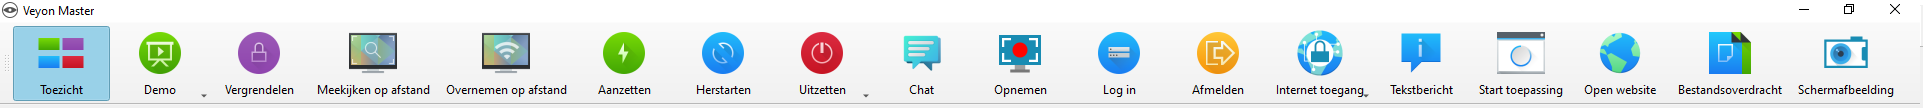
\includegraphics[width=1\textwidth]{graphics/SchermafbeeldingVeyonMasterInterface.png}
    \caption{Schermafbeelding interface Add-ons Veyon}
    \label{fig:Schermafbeelding interface Add-ons Veyon} 
\end{figure}

Binnen het programma ´Veyon Configurator´ biedt de sectie `Toegangscontrole internet´ de mogelijkheid tot configuratie van dit pakket. Na het voltooien wordt dit doorgestuurd naar Veyon Master, waar het wordt toegepast in de virtuele klasomgeving. De gebruiksvriendelijke interface van Veyon Master maakt het eenvoudig om de internettoegang voor de gehele klas of specifieke leerlingen aan of uit te zetten, zie figuur \ref{fig:Schermafbeelding Veyon Master internettoegang} en \ref{fig:Schermafbeelding Veyon Master internettoegang specifiek}.

\begin{figure}[h]
    \centering
    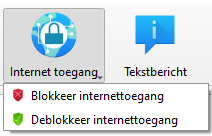
\includegraphics[width=0.55\textwidth]{graphics/SchermafbeeldingVeyonMasterInternettoegang.png}
    \caption{Schermafbeelding Veyon Master internettoegang}
    \label{fig:Schermafbeelding Veyon Master internettoegang} 
\end{figure}

\begin{figure}[h]
    \centering
    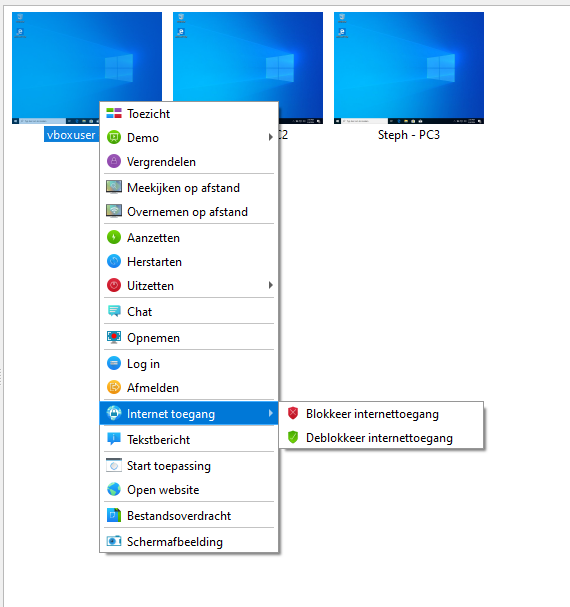
\includegraphics[width=0.5\textwidth]{graphics/SchermafbeeldingInternetToegangSpecifiek.png}
    \caption{Schermafbeelding Veyon Master internettoegang specifiek}
    \label{fig:Schermafbeelding Veyon Master internettoegang specifiek} 
\end{figure}\newpage

\subsection{Andere mogelijkheden}
Zoals duidelijk wordt weergegeven in de bovenstaande screenshots \ref{Implementatie Internet Access Control}, biedt Veyon de mogelijkheid om de gehele internettoegang flexibel te blokkeren en te deblokkeren. Het benadrukt de beperking bij het ontbreken van de optie om sociale media en E-commerce websites te blokkeren of te deblokkeren op een flexibele manier, wat niet voldoet aan de initiële verwachtingen van het programma.\newline

Anderzijds is het wel mogelijk om deze softwareoplossing verder te bespreken. Zodoende kan er besloten worden deze wel te gebruiken in de scholengroep IÑIGO om meer overzicht te bewaren ten opzichte van de leerlingen tijdens de lessen. Desondanks het niet mogelijk is om flexibele deblokkeringen en blokkeringen op sociale media en E-commerce websites te zetten. Veyon biedt nog andere mogelijkheden die de leerlingen hun opperste concentratie bij de lessen laat houden, ook al wordt er gebruik gemaakt van laptops of computers tijdens de lessen, namelijk:

\subsubsection{Monitoring}
Wanneer de Client pc's zijn opgestart, biedt Veyon Master de mogelijkheid om de schermen van leerlingen live te bekijken. Dit stelt leerkrachten in staat om toezicht te houden op de computers van hun leerlingen zonder zich alleen te beperken tot fysiek rondlopen in het klaslokaal. Door in realtime te kunnen waarnemen wat leerlingen op hun schermen doen, maakt deze functionaliteit het voor leerkrachten gemakkelijker en overzichtelijker om computers te gebruiken tijdens de lessen.

Vervolgens is de monitoringsfunctie van Veyon zeer nuttig tijdens het afnemen van een taak of toets. Dit omdat leerkrachten direct in staat zijn waar te nemen of leerlingen moeite hebben met de uitvoering van deze doelstellingen. Concluderend is het ook een gelegenheid de leerlingen te waarnemen wanneer er vrij wordt gesurft op het internet. Zodoende wordt het voor de leerling moeilijker om sociale media en E-commerce websites te bezoeken zonder weet van de leerkracht. 

Echter is het belangrijk op te merken dat deze monitoringsfunctie het meest efficiënt is wanneer de leerkracht de volledige aandacht besteed aan het bekijken van de Client-pc's. In andere situaties, kan deze functie minder efficiënt zijn.  

\subsubsection{Power mogelijkheden}
De power management functie van Veyon betrekt zich tot het opstarten, herstarten en afsluiten van één of meerdere Client pc's. Hoewel deze functie niet specifiek ontworpen is voor het beheer van sociale media en E-commerce websites, is het toch de moeite waard om kort te bespreken hoe deze functionaliteit indirecte invloed kan hebben op het beheer van dergelijke websites.

De power management functie kan bijvoorbeeld worden ingezet om Client pc's af te sluiten wanneer de desbetreffende leerling niet actief deelneemt aan de les. Dit biedt leerkrachten een effectieve manier om leerlingen een 'time-out' te geven wanneer zij herhaaldelijk met andere zaken bezig zijn dan met de leerstof. 

Daarnaast kan deze functie buiten de casus ook nuttig zijn in andere situaties, zoals het afsluiten van de Client pc's na afloop van de lessen of voor vakantieperiodes. Hiermee zorgt de leerkracht ervoor dat alle computers correct zijn afgesloten vooraleer de computers worden opgeborgen. Anderzijds kan deze functie dienen voor het opstarten van alle computers alvorens de leerlingen de klas betreden. Hierdoor kan bijvoorbeeld een toets direct van start gaan zonder veel tijd te verliezen aan opstartproblemen. Dit biedt een extra laag van beheer en controle over de informatica middelen binnen de scholengroep.
\subsubsection{Vergrendelmodus}

Hoewel de vergrendelmodus niet de meest geschikte oplossing is voor de flexibele activering en deactivering van sociale media en E-commerce websites, biedt het een uitstekende mogelijkheid voor algemene controle op Client pc's. Deze methode geeft leerkrachten de mogelijkheid om een de gehele klas of één computer volledig te vergrendelen, waardoor de leerlingen niets meer kunnen doen. \newline

De vergrendelmodus stelt de leerkracht in staat om via de Master pc een hele klas of specifieke Client pc's in vergrendeling te zetten. Wat betekent dat de leerkracht met één klik een groot slot op de computer van de selectie leerlingen kan plaatsen, waardoor verder werken onmogelijk wordt op de desbetreffende computer. Deze vergrendeling blijft actief totdat de leerkracht via de Master pc dit opheft. Dit kan worden waargenomen in onderstaande screenshot \ref{fig:Schermafbeelding Veyon Client vergrendel} en voor de master pc \ref{fig:Schermafbeelding Veyon Master vergrendel}

\begin{figure}[h]
    \centering
    
\includegraphics[width=0.5\textwidth]{graphics/Schermafbeelding vergrendeling client.png}
    \caption{Schermafbeelding Veyon Client vergrendel}
    \label{fig:Schermafbeelding Veyon Client vergrendel} 
\end{figure}

\begin{figure}[h]
    \centering
    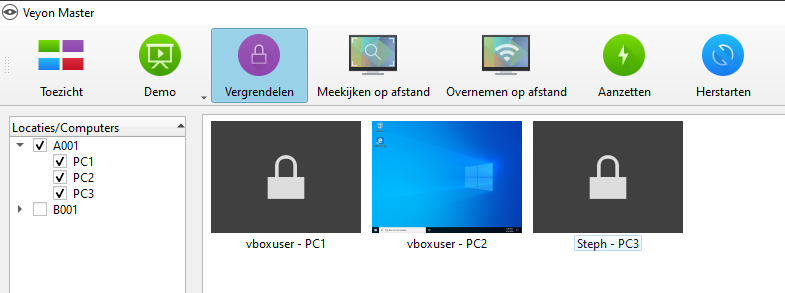
\includegraphics[width=0.5\textwidth]{graphics/SchermafbeeldingvergrendelmodusMaster.png}
    \caption{Schermafbeelding Veyon Master vergrendel}
    \label{fig:Schermafbeelding Veyon Master vergrendel} 
\end{figure}

Zoals eerder vernoemd biedt Veyon tal van extra opties om de concentratie van de leerlingen te verhogen en de supervisie van de leerkracht te verbeteren. Ook toont deze proof of concept overtuigend aan dat Veyon een waardevolle tool is voor het beheren van klaslokalen in de scholengroep IÑIGO, noch deze voldoet aan de vooropgestelde verwachtingen van de flexibiliteit van activering en deactivering van sociale media en E-commerce websites. Toch levert de grote flexibiliteit van het programma, gecombineerd met de grote hoeveelheid aan mogelijkheden en features, Veyon tot een zeer aantrekkelijke speler in de wereld van Classroom management software tools.

